\documentclass[]{elsarticle} %review=doublespace preprint=single 5p=2 column
%%% Begin My package additions %%%%%%%%%%%%%%%%%%%
\usepackage[hyphens]{url}

  \journal{A Journal of Imaginary Results} % Sets Journal name


\usepackage{lineno} % add
\providecommand{\tightlist}{%
  \setlength{\itemsep}{0pt}\setlength{\parskip}{0pt}}

\usepackage{graphicx}
\usepackage{booktabs} % book-quality tables
%%%%%%%%%%%%%%%% end my additions to header

\usepackage[T1]{fontenc}
\usepackage{lmodern}
\usepackage{amssymb,amsmath}
\usepackage{ifxetex,ifluatex}
\usepackage{fixltx2e} % provides \textsubscript
% use upquote if available, for straight quotes in verbatim environments
\IfFileExists{upquote.sty}{\usepackage{upquote}}{}
\ifnum 0\ifxetex 1\fi\ifluatex 1\fi=0 % if pdftex
  \usepackage[utf8]{inputenc}
\else % if luatex or xelatex
  \usepackage{fontspec}
  \ifxetex
    \usepackage{xltxtra,xunicode}
  \fi
  \defaultfontfeatures{Mapping=tex-text,Scale=MatchLowercase}
  \newcommand{\euro}{€}
\fi
% use microtype if available
\IfFileExists{microtype.sty}{\usepackage{microtype}}{}
\bibliographystyle{elsarticle-harv}
\usepackage{graphicx}
% We will generate all images so they have a width \maxwidth. This means
% that they will get their normal width if they fit onto the page, but
% are scaled down if they would overflow the margins.
\makeatletter
\def\maxwidth{\ifdim\Gin@nat@width>\linewidth\linewidth
\else\Gin@nat@width\fi}
\makeatother
\let\Oldincludegraphics\includegraphics
\renewcommand{\includegraphics}[1]{\Oldincludegraphics[width=\maxwidth]{#1}}
\ifxetex
  \usepackage[setpagesize=false, % page size defined by xetex
              unicode=false, % unicode breaks when used with xetex
              xetex]{hyperref}
\else
  \usepackage[unicode=true]{hyperref}
\fi
\hypersetup{breaklinks=true,
            bookmarks=true,
            pdfauthor={},
            pdftitle={An Example of a Term Paper},
            colorlinks=false,
            urlcolor=blue,
            linkcolor=magenta,
            pdfborder={0 0 0}}
\urlstyle{same}  % don't use monospace font for urls

\setcounter{secnumdepth}{0}
% Pandoc toggle for numbering sections (defaults to be off)
\setcounter{secnumdepth}{0}
% Pandoc header
\usepackage{booktabs}
\usepackage{longtable}
\usepackage{array}
\usepackage{multirow}
\usepackage{wrapfig}
\usepackage{float}
\usepackage{colortbl}
\usepackage{pdflscape}
\usepackage{tabu}
\usepackage{threeparttable}
\usepackage{threeparttablex}
\usepackage[normalem]{ulem}
\usepackage{makecell}
\usepackage{xcolor}



\begin{document}
\begin{frontmatter}

  \title{An Example of a Term Paper}
    \author[School of Geography and Earth Sciences]{Antonio Paez\corref{c1}}
   \ead{paezha@mcmaster.ca} 
   \cortext[c1]{Corresponding Author}
      \address[School of Geography and Earth Sciences]{McMaster University, 1280 Main St W, Hamilton, ON, L8S 4K1 Canada}
  
  \begin{abstract}
  This is an example of a paper created using the package
  \texttt{rticles}. It is an example of the final deliverable in the
  course GEO 712 Reproducible Research Workflow. The objective of the
  paper is to put into practice skills learned in the course, in the form
  of a self-contained, reproducible document in the format of a journal
  article.
  
  Notice that for this paper, the instructors will not evaluate the
  research per se, but rather the reproducibility of the research.
  \end{abstract}
  
 \end{frontmatter}

\hypertarget{introduction}{%
\section{Introduction}\label{introduction}}

The economy of a nation is tied to its consumption of energy, since
every process of production requires energy as an input (Warr et al.,
2010). However, the strength of the relationship between the economy and
the consumption of energy varies. Some countries were more successful
than others in terms of decoupling their productive processes from
energy after the oil shocks of the 1970s (MacKillop, 1989). This was
achieved by increasing the efficiency of production, so that the same
output could be produced using less energy, or in somewhat different
terms, by improving their energy intensity.

The relationship between economic output and energy consumption is of
interest at a time when the effects of a carbon-intense economy is
creating a heavy environmental burden. A relevant question is, what
countries are more energy-efficient, and can we learn from them. To
explore this question we will consider data on national energy use (in
barrels of oil per day), economic output (GDP), and \(CO_2\) emissions.

\hypertarget{exploratory-data-analysis}{%
\section{Exploratory Data Analysis}\label{exploratory-data-analysis}}

Data were collected from a variety of sources as documented in the
package \texttt{packr} (see
{[}paezha/Reproducible-Research-Workflow/Session-07-Creating-R-Packages-and-Documenting-Data/packr{]}).
The summary statistics of the data appear in Table
\ref{tab:descriptive-statistics}. Very large disparities can be observed
in terms of all indicators of interest: while some countries have a GDP
per capita measures in hundreds of dollars, others measure their GDP per
capita in tens of thousands of dollars. Similarly, the difference in
consumption of oil between the country with the lowest to the highest
use of this resource is three orders of magnitude higher. The table also
illustrates how emissions of \(CO_2\) for the worst polluters increased
by a factor of two between 1995 and 2015; emissions at the bottom, in
contrast, increased by a factor of approximately 1.5 in the same period
of time.

\begin{table}

\caption{\label{tab:descriptive-statistics-7}\label{tab:descriptive-statistics} Descriptive statistics: energy and emissions of world countries}
\centering
\resizebox{\linewidth}{!}{
\begin{tabular}[t]{lrrrrrr}
\toprule
Statistic & \makecell[c]{Population\\(millions)} & GDP per capita & \makecell[c]{Energy use\\(millions of \\barrels per day)} & \makecell[c]{CO2 1995\\(millions ton)} & \makecell[c]{CO2 2005\\(millions ton)} & \makecell[c]{CO2 2015\\(millions ton)}\\
\midrule
\rowcolor{gray!6}  Mean & 38.466 & 13572.01 & 0.491 & 0.121 & 0.153 & 0.185\\
Min & 0.005 & 145.00 & 0.000 & 0.000 & 0.000 & 0.000\\
\rowcolor{gray!6}  Max & 1379.303 & 100161.00 & 19.530 & 5.295 & 6.175 & 10.642\\
Standard Deviation & 142.048 & 18550.58 & 1.752 & 0.489 & 0.649 & 0.892\\
\bottomrule
\end{tabular}}
\end{table}

Figure \ref{fig:energy-to-gdp} is a scatterplot of energy consumption to
GPD. It can be seen that in general, greater economic output is
associated with greater consumption of energy. However, there are some
important differences. If we fit a regression line to this relationship,
the line would indicate the \emph{expected} economic output for a given
level of energy consumption. Points below the line would use more energy
for a lower level of economic output than expected, whereas points above
the line would represent greater economic output than expected, given
their energy consumption.

\begin{figure}
\centering
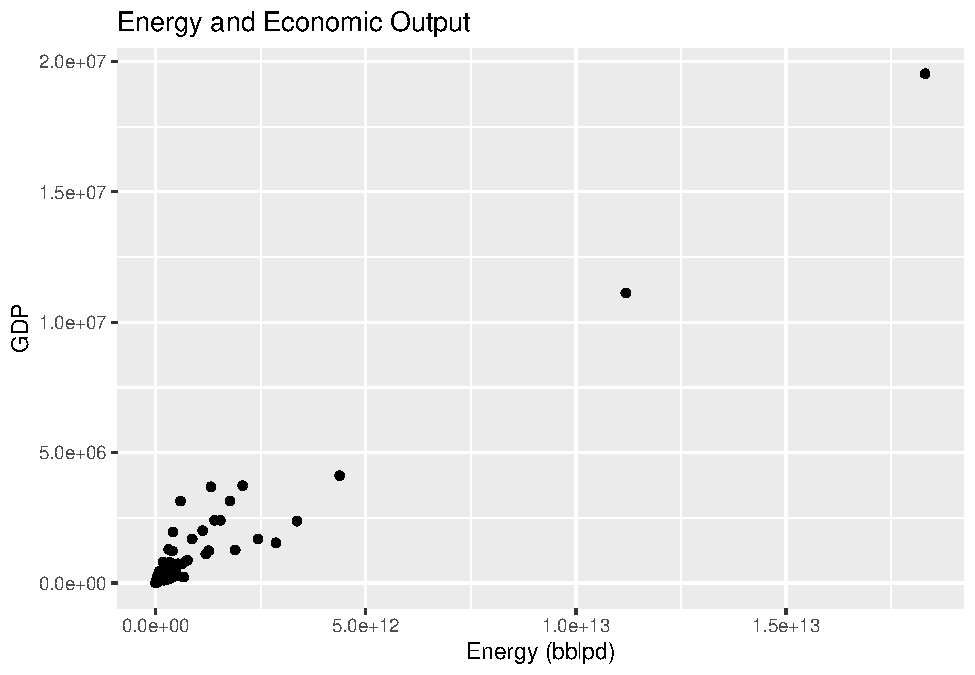
\includegraphics{Elsevier-Template_files/figure-latex/fig-energy-to-gdp-1.pdf}
\caption{\label{fig:energy-to-gdp} The relationship between energy
consumption and economic output by world countries}
\end{figure}

The regression line is estimated as follows: \[
GDP_i = \beta_0 + \beta_1\text{bblpd}_i + \epsilon_i
\]

This is a linear model and can be estimated using ordinary least
squares. The scatterplot of energy to GDP with this line is shown in
Figure \ref{fig:energy-to-gdp-with-line}. Clearly, some countries are
more efficient than others in that they can produce more with less
energy. The more a point deviates from the regression line, the more
efficient that economy is. It would be interesting to

\begin{figure}
\centering
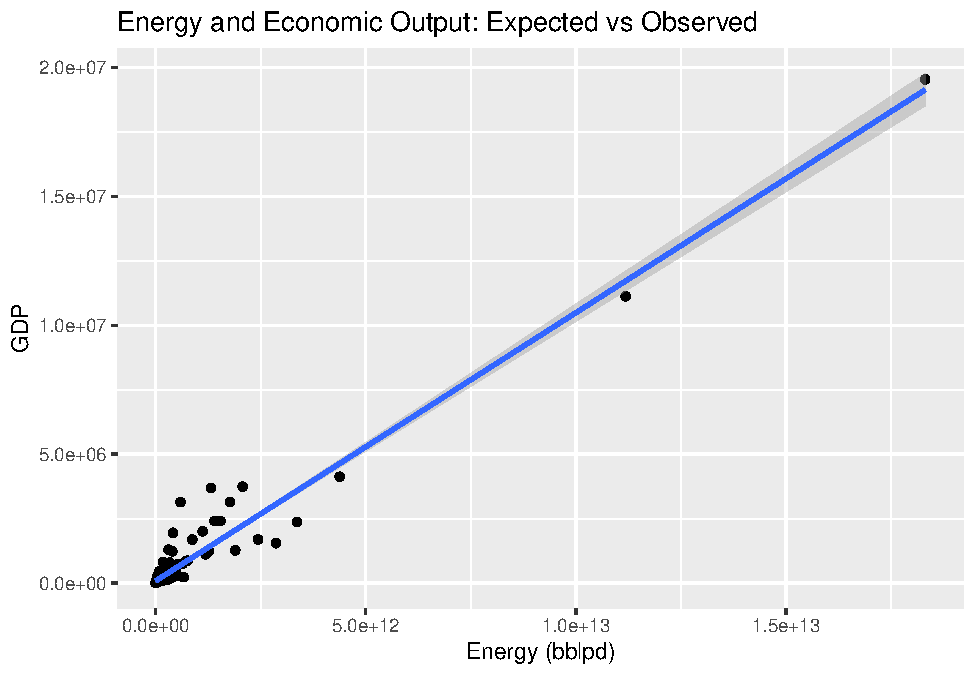
\includegraphics{Elsevier-Template_files/figure-latex/fig-energy-to-gdp-with-line-1.pdf}
\caption{\label{fig:energy-to-gdp-with-line} A regression line gives the
expected values of GDP given energy consumption}
\end{figure}

Figure \ref{fig:right-left-panel-plot} shows Figures
\ref{fig:energy-to-gdp} and \ref{fig:energy-to-gdp-with-line} side by
side.

\begin{figure}
\centering
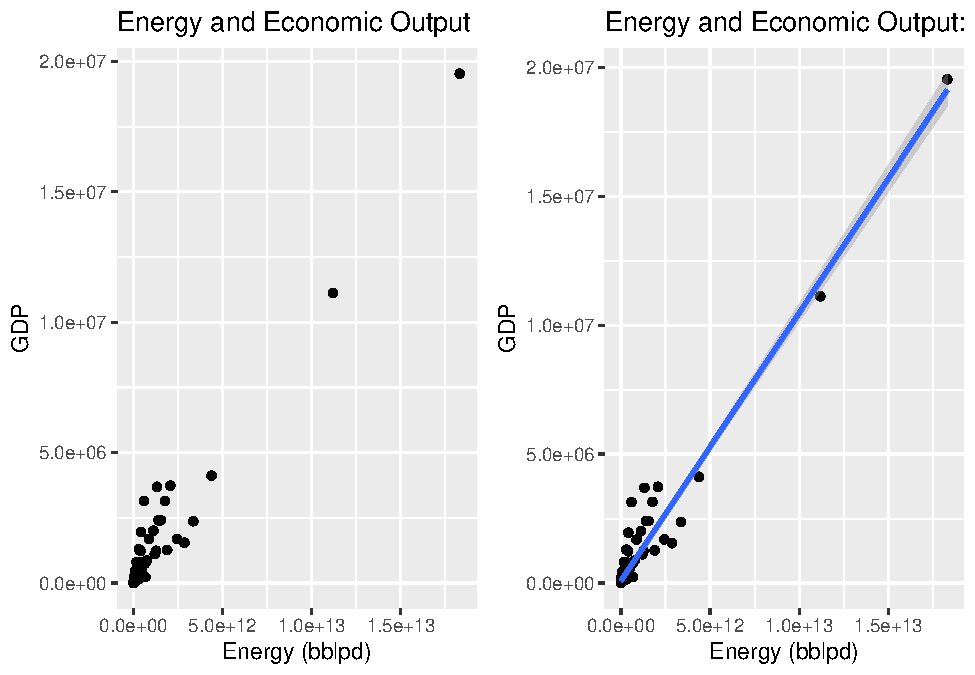
\includegraphics{Elsevier-Template_files/figure-latex/fig-right-left-panel-plot-1.pdf}
\caption{\label{fig:right-left-panel-plot} Two plots in a single figure;
left panel is Figure 1 and right panel is Figure 2}
\end{figure}

Figure \ref{fig:top-bottom-panel-plot} shows Figures
\ref{fig:energy-to-gdp} and \ref{fig:energy-to-gdp-with-line} as a
two-panel figure with one column and two rows.

\begin{figure}
\centering
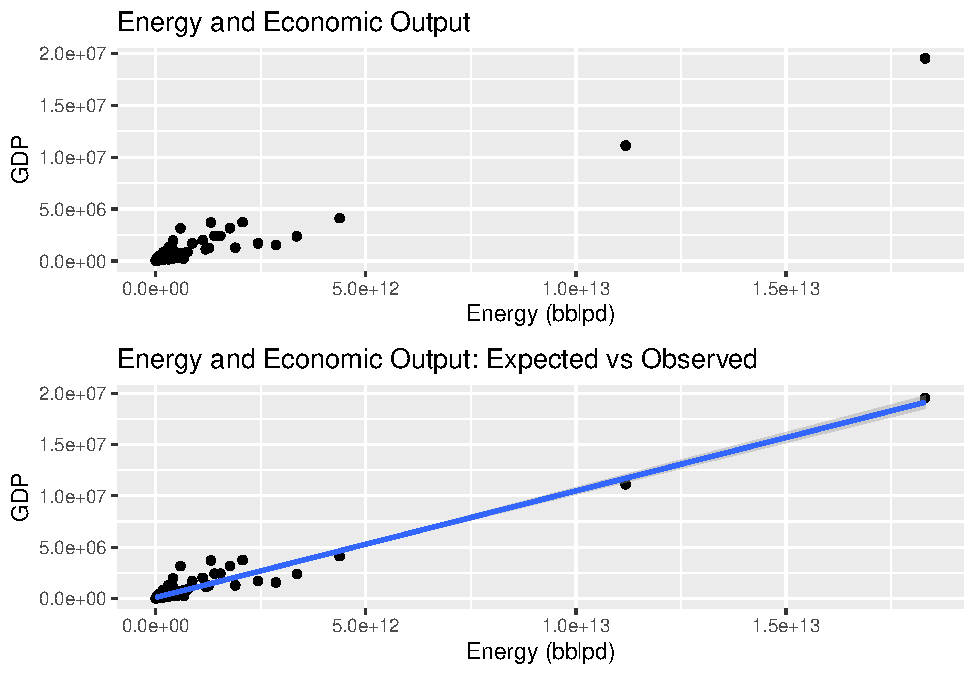
\includegraphics{Elsevier-Template_files/figure-latex/fig-top-bottom-panel-plot-1.pdf}
\caption{\label{fig:top-bottom-panel-plot} Two plots in a single figure;
top panel is Figure 1 and bottom panel is Figure 2}
\end{figure}

Another question of interest is the way energy is related to the
emission of Greenhouse Gases (GHG), particularly \(CO_2\). Figure
\ref{fig:gdp-emissions-by-year} shows that for some countries, emissions
increased over time more than proportionally relative to GDP.

\begin{figure}
\centering
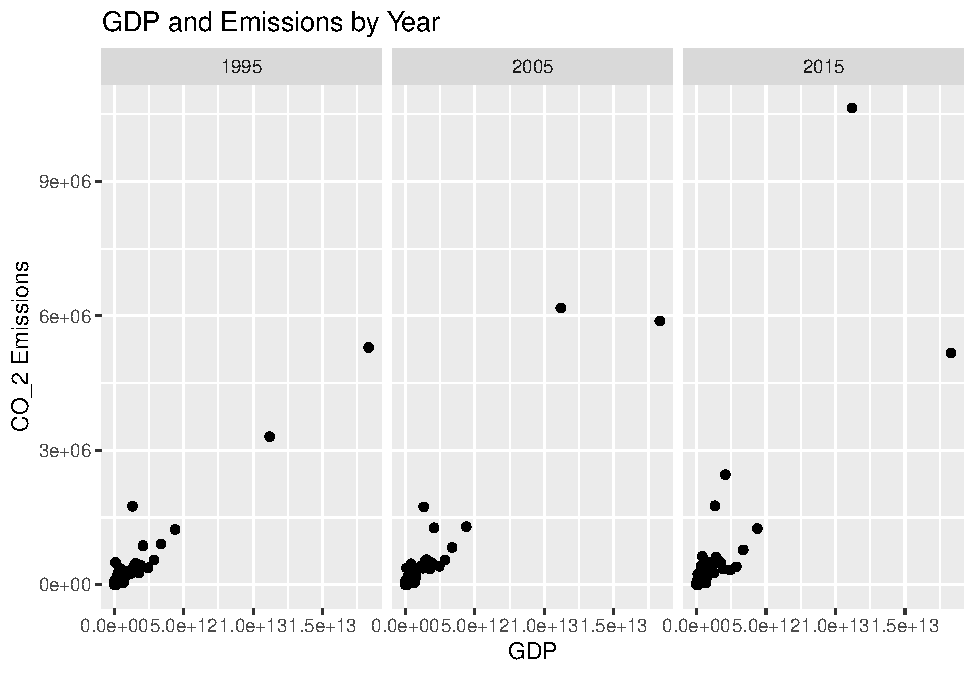
\includegraphics{Elsevier-Template_files/figure-latex/fig-gdp-emissions-by-year-1.pdf}
\caption{\label{fig:gdp-emissions-by-year} CO\_2 emissions versus GDP by
year}
\end{figure}

\hypertarget{modelling}{%
\section{Modelling}\label{modelling}}

\hypertarget{references}{%
\section*{References}\label{references}}
\addcontentsline{toc}{section}{References}

\hypertarget{refs}{}
\leavevmode\hypertarget{ref-Mackillop1989decoupling}{}%
MacKillop, A., 1989. Decoupling---recoupling and oil shock. Energy
Policy 17, 311--322.

\leavevmode\hypertarget{ref-Warr2010energy}{}%
Warr, B., Ayres, R., Eisenmenger, N., Krausmann, F., Schandl, H., 2010.
Energy use and economic development: A comparative analysis of useful
work supply in austria, japan, the united kingdom and the us during 100
years of economic growth. Ecological Economics 69, 1904--1917.


\end{document}


